\documentclass[11pt,aps,preprint,nofootinbib,superscriptaddress,tightenlines]{revtex4-2}
\usepackage[T1]{fontenc}
\usepackage{amsmath,amssymb,mathtools}
\let\lambdabar\relax   % revtex defines it; newpxmath does too
\usepackage{newpxtext,newpxmath}
\usepackage{bm}
\usepackage[final]{microtype}
\usepackage{xcolor}
\usepackage{booktabs}
\usepackage{graphicx}
\usepackage{dsfont}
\usepackage[most]{tcolorbox}
\usepackage{algpseudocode}
\newcommand{\one}{\mathds{1}}
\newcommand{\avg}[1]{\langle #1\rangle}
\newcommand{\klab}{\mathcal B}
\definecolor{darkblue}{RGB}{20,60,140}
\definecolor{accent}{RGB}{30,80,150}
\definecolor{tint}{RGB}{243,246,251}
\newtcolorbox{algobox}[1]{enhanced, colback=tint, colframe=accent, boxrule=0.6pt, arc=2pt,
  left=6pt, right=6pt, top=4pt, bottom=4pt, fonttitle=\bfseries\small, coltitle=white,
  colbacktitle=accent, title={#1}, before skip=10pt, after skip=10pt}
\newtcolorbox{keyeq}{enhanced, colback=tint, frame hidden, borderline west={2pt}{0pt}{accent},
  sharp corners, left=4pt, right=4pt, top=0pt, bottom=0pt, before skip=6pt, after skip=6pt}
\usepackage[colorlinks=true,linkcolor=darkblue,citecolor=darkblue,urlcolor=darkblue]{hyperref}

\def\st{\begin{equation}}
\def\stp{\end{equation}}
\def\Eq#1{eq.~(\ref{#1})}
\def\Sect#1{Sect.~\ref{#1}}
\def\Fig#1{Fig.~\ref{#1}}
\def\App#1{Appendix~\ref{#1}}
\def\tr{\operatorname{tr}}
\let\oldparagraph\paragraph
\renewcommand{\paragraph}{\par\bigskip\oldparagraph}

\begin{document}
\sloppy

\title{The renormalized Hamiltonian as a Legendre transform:\\ development plan}
\author{D.~Teaney}
\affiliation{Department of Physics and Astronomy, Stony Brook University,
Stony Brook, New York 11794, USA}
\date{\today}

\begin{abstract}
A plan for implementing, testing and measuring the renormalized particle Hamiltonian defined as the Legendre transform of the wanted single-particle
free energy, for a constant speed of sound (not necessarily conformal), in the default scheme of the code.  Written on 2026-11-22 for a session at
NERSC to carry out over a day or so.  The derivation and the single-particle checks are in \nolinkurl{partition.tex}, Appendix ``Notes from
discussion'' (subsections from ``The label $s_{\rm eff}$'' to ``Implementation plan for the root finding''); the theory of the counterterm is in
\nolinkurl{partition_v2.tex}, Sects.~``Equilibrium in motion'' and ``The counterterms: formal structure''.
\end{abstract}

\maketitle
\tableofcontents

%=============================================================================
\section{The goal}
\label{sec:goal}

The model's particles carry a label $s_a$ (entropy), a momentum $\bm m_a$ and a volume $V_a$ ($=1/n_a$ in the default $n$-scheme).  At one loop the
canonical ensemble of the present (tree-level) Hamiltonian has the target fluid's thermodynamics plus terms of order $T$ per particle: the label gas
and the fluctuations of each particle.  The renormalized Hamiltonian removes them.  The present option \texttt{SPH\_RENORM=1} does it for the conformal
fluid at rest by a shift of the entropy alone; it leaves the sound term in motion (the violation $R$ of the density-frame relation, a deficit of the
momentum susceptibility) and it cannot treat a non-conformal equation of state.

The new definition: the Hamiltonian of a particle is the Legendre transform of the free energy we want at tree level,
\begin{keyeq}
\st
\begin{gathered}
F_{\rm want}(T,\bm v,V)=F_{\rm t}(T,\bm v,V)+T\,\delta\ln Z_1(T,\bm v,V),\\
H_a(s,\bm m,V)=F_{\rm want}+Ts+\bm v\cdot\bm m\quad\text{at}\quad s=-\frac{\partial F_{\rm want}}{\partial T},\quad \bm m=-\frac{\partial F_{\rm want}}{\partial\bm v},
\end{gathered}
\label{Hdef}
\stp
\end{keyeq}
with $F_{\rm t}=-p(T_{\rm rel})V$ the target and $\delta\ln Z_1$ the excess of the tree-level model's $\ln Z_1$ over the target's.  The tree level of $H_a$ is
$F_{\rm want}$ exactly, and its one loop removes $\delta\ln Z_1$; the target's thermodynamics remains, up to $O(T/s_a)$ per particle.  The transform divides
the counterterm between $s$ and $\bm m$ by itself, gives $\partial H/\partial s=T$ and $\partial H/\partial\bm m=\bm v$ exactly ($|\dot{\bm x}|<1$), and treats a
non-conformal equation of state with no change.  Checked by the exact single-particle quadrature (\Sect{sec:refs}).

\paragraph{The deliverable.}  When the owner comes back: the option implemented and tested, its speed measured, and the renormalization demonstrated by
repeating the measurements of the campaign \texttt{eos\_renorm} at rest (\nolinkurl{gravity.tex}, ``Results'': $E$, $P$, the trace, $dE/dT$, $dP/dT$, $c_s^2$,
$S(k)$), now for the Legendre Hamiltonian and for $c_s^2=1/2$ and $1/4$, and by the same measurements at $v=0.8$ together with the momentum and the
density-frame relation $R$ (\Sect{sec:campaign}).

Apart from the two maps between the particle's variables and its state, the code is unchanged: the integrators, the stochastic step and its
Hastings correction, hybrid Monte Carlo and the measurements use the particle's $T$, $\bm v$, pressure and energy as now.

%=============================================================================
\section{The formulas}
\label{sec:formulas}

\paragraph{General.}  With $T$ the bare (density-frame) temperature, $T_{\rm rel}=\gamma T$, $w$ and $c_s^2$ at $T_{\rm rel}$, $d$ dimensions and the bulk modulus
of the labels $\klab$,
\st
\delta\ln Z_1=\tfrac{d+1}2\ln\big(2\pi V\gamma\,wT_{\rm rel}\big)+\tfrac12\ln\big(1-c_s^2v^2\big)-\tfrac12\ln c_s^2-\ln T+(1-\klab)\ln V+1 .
\label{dlnZ}
\stp
Here: $\klab=0$ (neutral labels), and the constant $1$ makes $\mu/T=0$.

\paragraph{Implementation: constant $c_s^2$, $d=2$.}  The code's \texttt{ConstantCs2EOS}, $T_{\rm rel}=T_{\rm scale}\,e^{c_s^2/(1+c_s^2)}$, is
\st
p=A\,T_{\rm rel}^{\,n},\qquad n=1+\frac1{c_s^2},\qquad A=c_s^2\,T_{\rm scale}^{-n},\qquad w=n\,p .
\stp
Then, with $(T,v)$ as the independent variables and $\gamma=(1-v^2)^{-1/2}$,
\begin{keyeq}
\st
F_{\rm want}=-A\,V(\gamma T)^n+T\,\Delta,\qquad
\Delta=\tfrac52\ln V+\tfrac52\ln\gamma+k\ln(\gamma T)+\tfrac12\ln\big(1-c_s^2v^2\big)+C ,
\label{Fwant}
\stp
\end{keyeq}
\st
k=2+\frac3{2c_s^2},\qquad C=\tfrac32\ln(2\pi nA)-\tfrac12\ln c_s^2+1 .
\stp
The Legendre pair, the energy and the particle's pressure:
\begin{align}
s&=nAV\gamma^nT^{n-1}-\Delta-k , \label{s}\\
|\bm m|&=nAVT^n\gamma^{n+2}v-T\,v\Big[\big(\tfrac52+k\big)\gamma^2-\frac{c_s^2}{1-c_s^2v^2}\Big],\qquad \hat{\bm m}=\hat{\bm v} , \label{m}\\
H&=F_{\rm want}+Ts+v|\bm m| , \label{H}\\
P&\equiv-\frac{\partial H}{\partial V}\Big|_{s,\bm m}=-\frac{\partial F_{\rm want}}{\partial V}\Big|_{T,v}=A(\gamma T)^n-\frac52\,\frac TV . \label{P}
\end{align}
The first terms of $s$ and $|\bm m|$ are the target's, $\gamma s(T_{\rm rel})V$ and $w\gamma^2vV$.  The Jacobian of $(s,|\bm m|)$ with respect to $(T,v)$ (the
particle's susceptibility; symmetric by the Maxwell relation $\partial s/\partial v=\partial|\bm m|/\partial T$), with $K=\tfrac52+k$ and $q=1-c_s^2v^2$:
\begin{align}
\frac{\partial s}{\partial T}&=n(n-1)AV\gamma^nT^{n-2}-\frac kT ,\\
\frac{\partial s}{\partial v}=\frac{\partial|\bm m|}{\partial T}&=n^2AVT^{n-1}\gamma^{n+2}v-K\gamma^2v+\frac{c_s^2v}q ,\\
\frac{\partial|\bm m|}{\partial v}&=nAVT^n\gamma^{n+2}\big(1+(n+2)\gamma^2v^2\big)-T\Big[K\big(\gamma^2+2\gamma^4v^2\big)-\frac{c_s^2(1+c_s^2v^2)}{q^2}\Big] .
\end{align}
For the inverse map (votes) the residual $e-H$ replaces $s-s(T,v)$; since $\partial H/\partial T=T\,\partial s/\partial T+v\,\partial|\bm m|/\partial T$ and
$\partial H/\partial v=T\,\partial s/\partial v+v\,\partial|\bm m|/\partial v$ (from $dH=T\,ds+v\,d|\bm m|$), its Jacobian follows from the same entries.

\paragraph{What the code needs from a solve.}  In the $n$-scheme the forces use $p_aV_a^2$, the velocity is local, $T_{\rm eff}=T$ (\nolinkurl{src/ideal.jl}).
So the forward solve fills the present fields:
\st
\begin{gathered}
\texttt{pa.p}\leftarrow P,\qquad \texttt{pa.T}\leftarrow T,\qquad \texttt{pa.}\gamma\leftarrow\gamma,\\
\texttt{pa.v\_over\_S}\leftarrow\frac{\bm v}{S_a},\qquad \texttt{pa.H\_over\_S}\leftarrow\frac{H}{s_a} .
\end{gathered}
\stp

\paragraph{Reference values.}  From \nolinkurl{examples/renorm_quadrature_legendre.py} (\texttt{Model(c2).legendre}), $T_{\rm scale}=1$, for the unit tests:
\begin{center}
\small
\resizebox{\linewidth}{!}{\begin{tabular}{cccccccc}
\toprule
$c_s^2$ & $T$ & $v$ & $V$ & $s$ & $|\bm m|$ & $H$ & $P$ \\
\midrule
$0.5$ & $3.0$ & $0$ & $4.0$ & $3.5329615802\times10^{1}$ & $0$ & $9.3000000000\times10^{1}$ & $1.1625000000\times10^{1}$ \\
$0.5$ & $3.0$ & $0.8$ & $4.0$ & $2.2769125486\times10^{2}$ & $1.6184313725\times10^{3}$ & $1.7797450980\times10^{3}$ & $6.0625000000\times10^{1}$ \\
$0.5$ & $1.7$ & $0.95$ & $0.5$ & $5.2134000814\times10^{1}$ & $1.0565293387\times10^{3}$ & $1.0758910379\times10^{3}$ & $7.2188166117\times10^{1}$ \\
$0.25$ & $3.0$ & $0$ & $1.0$ & $7.9676423584\times10^{1}$ & $0$ & $2.1900000000\times10^{2}$ & $5.3250000000\times10^{1}$ \\
$0.25$ & $3.0$ & $0.8$ & $1.0$ & $1.2752332646\times10^{3}$ & $8.6112698413\times10^{3}$ & $9.9900158730\times10^{3}$ & $7.7375000000\times10^{2}$ \\
$0.25$ & $1.7$ & $0.95$ & $0.5$ & $1.7311977590\times10^{3}$ & $2.8956034219\times10^{4}$ & $2.9886312509\times10^{4}$ & $1.1873400004\times10^{3}$ \\
\bottomrule
\end{tabular}}
\end{center}

%=============================================================================
\section{The work, in order}
\label{sec:work}

Branch: \texttt{legendre} (created from \texttt{statics} with this note; \texttt{git fetch; git checkout legendre}).  Read \nolinkurl{nersc/LOG.md}, \nolinkurl{CLAUDE.md}, this note, and the subsections of
\nolinkurl{partition.tex} named in the abstract.  Follow \nolinkurl{CLAUDE.md}: no simulations on the login node beyond seconds, \texttt{julia --project=nersc},
output under \texttt{\$SCRATCH/sph/}, never commit \texttt{.jls}/\texttt{.h5}.

\subsection{A. Route the particle-level maps through two functions (no change of numerics)}
\label{sec:routing}

The target's particle-level maps are called in about 35 places; find them with a search of \texttt{src/*.jl} for \texttt{eos\_newton}, \texttt{eos\_from\_energy},
\texttt{particle\_energy(}, \texttt{particle\_entropy(}, \texttt{particle\_entropy\_lnT(} and \texttt{rest\_energy(}:
\nolinkurl{src/stochastic.jl} (13), \nolinkurl{src/measure.jl} (11), \nolinkurl{src/viscous.jl} (4, the back map), \nolinkurl{src/pointwise.jl},
\nolinkurl{src/hmc.jl}, \nolinkurl{src/grid.jl}, \nolinkurl{src/sph.jl} (\texttt{solve\_eos!}).
\begin{enumerate}
\item Define two functions with the present behaviour: the \emph{forward} map, $(s,\bm m,V)\to$ the particle's state (what \texttt{solve\_eos!} and
  \texttt{particle\_energy} compute), and the \emph{inverse} map, $(e,\bm m,V)\to$ the entropy $S$ (and $T$, $\bm v$), what \texttt{eos\_from\_energy},
  \texttt{particle\_entropy} and \texttt{particle\_entropy\_lnT} compute.
\item Replace every particle-level call by one of the two.  Leave field-level (density) uses that are not about a particle alone as they are, and list them.
\item \texttt{test/run.sh all}: unit tests pass, scripts load, and the regression against \texttt{main} is bit-identical (the known exception: the
  \texttt{hast\_lq\_*} datasets differ run to run, thread order; \nolinkurl{nersc/LOG.md}).  If anything else differs, stop and find why.
\end{enumerate}

\subsection{B. The new maps: \texorpdfstring{\nolinkurl{src/renorm.jl}}{src/renorm.jl}}
\label{sec:renormjl}

\begin{itemize}
\item $F_{\rm want}$ and the entries of \Sect{sec:formulas} for \texttt{ConstantCs2EOS} (any $c_s^2$), $d=2$, $\klab=0$; error for other equations of state and
  dimensions.  Write them in the unknowns $(\ln T_{\rm rel},\eta)$, $\gamma=\cosh\eta$, $\gamma v=\sinh\eta$, or in $(T,v)$ with care near $\gamma_{\max}=100$
  (\texttt{SPH\_GAMMA\_MAX}): the rapidity avoids the cancellation in $1-v^2$ and keeps every Newton step in the domain.
\item \texttt{renorm\_state(s, m, V, eos; guess)}: solve \Eq{s}, \Eq{m} for $(T,v)$ by Newton with the analytic Jacobian; return $T$, $\bm v$ (along $\bm m$),
  $\gamma$, $H$, $P$.
\item \texttt{renorm\_entropy(e, m, V, eos; guess)}: solve $H(T,v)=e$ and \Eq{m} for $(T,v)$; return $S$ from \Eq{s}, $T$, $\bm v$.  The vote's weight with the
  Liouville measure is $S-\ln T$ (as \texttt{particle\_entropy\_lnT}).
\item Newton: stop at a relative residual $10^{-14}$ (both equations), at most 8 iterations; halve a step that increases the residual; count the failures in a
  guard counter (as \texttt{GUARD\_REJECTED} in \nolinkurl{src/stochastic.jl}) and return $-\infty$ for the vote, \texttt{NaN} for the state, if a solve fails.
\item Starting points, in order of preference: (i) the particle's stored state from the last solve (warm start; store $\ln T_{\rm rel}$ and $\eta$, in
  \texttt{pa.e} and from \texttt{pa.}$\gamma$, or in two new fields of \texttt{Particle}); (ii) for a vote's proposal, the current state of the particle;
  (iii) cold: the target's closed-form solve (\texttt{rest\_energy}, or the forward map through $|\bm m|/s^{n/(n-1)}$, a function of $v$ alone), at the entropy
  shifted by $\Delta+k$ of \Eq{s} evaluated there, then Newton.
\end{itemize}

\begin{algobox}{Forward solve (one particle)}
\begin{algorithmic}[1]
\State Take the start: the stored $(\ln T_{\rm rel},\eta)$ if there is one, else the target's solution at the shifted entropy.
\Repeat
  \State From $(T,v)$ evaluate $s(T,v)$ and $|\bm m|(T,v)$ by \Eq{s}, \Eq{m}, and the Jacobian.
  \State Solve the $2\times2$ linear system for the step that zeroes the residuals $s-s_a$ and $|\bm m|-|\bm m_a|$.
  \State Take the step; if the residual grew, halve it until it does not.
\Until{both relative residuals are below $10^{-14}$, or 8 iterations (then count a failure)}
\State Return $T$, $\bm v=v\,\hat{\bm m}_a$, $\gamma$, $H$ by \Eq{H}, $P$ by \Eq{P}; store $(\ln T_{\rm rel},\eta)$ for the next call.
\end{algorithmic}
\end{algobox}

\subsection{C. The switch}
\label{sec:switch}

\begin{itemize}
\item \texttt{SPH\_RENORM=legendre}, chosen at load time as \texttt{SPH\_RENORM=1} is now (methods defined under \texttt{if}), so that with it off the code is
  exactly that of before.  Keep \texttt{SPH\_RENORM=1} working.
\item With the switch on: the forward and the inverse functions of \Sect{sec:routing} call \texttt{renorm\_state} and \texttt{renorm\_entropy}.
\item Errors (not silent fallbacks) for: $\texttt{volume}\neq\texttt{:number}$ or $\texttt{hamiltonian}\neq\texttt{:energy}$ (in the entropy-volume scheme $H/s$
  also serves as $\partial H/\partial s$, which fails for a non-extensive $H$); $d\neq2$; an equation of state other than \texttt{ConstantCs2EOS}; the Einstein
  measure (the Liouville measure is needed, as for \texttt{SPH\_RENORM=1}).
\item The viscous step's back map and the measurements go through the same two functions; check that the energy reported by \texttt{energy\_pressure}
  is $\sum_aH_a$ and that it uses \texttt{pa.p}$=P$.
\end{itemize}

\subsection{D. Tests (\texttt{test/})}
\label{sec:tests}

\begin{enumerate}
\item The reference values of \Sect{sec:formulas}, to $10^{-10}$ relative.
\item The Legendre identities by central differences: $\partial H/\partial s=T$, $\partial H/\partial\bm m=\bm v$, $\partial H/\partial V=-P$.
\item Forward and inverse are inverses: $H(S(e,\bm m,V),\bm m,V)=e$ to $10^{-13}$, on a grid of $s_a\in[10,10^4]$, $\gamma\in[1,100]$, two values of $c_s^2$.
\item With the counterterm set to zero ($\Delta+k\to0$ and the $T$-terms of $|\bm m|$ off) the new solves reproduce the target's (\texttt{eos\_newton},
  \texttt{eos\_from\_energy}) to roundoff.
\item Warm and cold starts give the same answer; count the iterations (expect 1--2 warm, 2--4 cold).
\item \texttt{test/run.sh all} with the switch off: bit-identical (as in A); with it on: the unit tests pass and every script loads.
\end{enumerate}

\subsection{E. Speed}
\label{sec:speed}

Measure before and after (\texttt{BenchmarkTools}, \texttt{julia -t 8}): one step of the ideal integrator (generalized leapfrog) and one sweep of the stochastic
step, $N\approx10^4$, $s_a=54$, $c_s^2=1/2$; and one update of hybrid Monte Carlo at $N=360$.  Record: time per step, the share in the solves, the mean
number of Newton iterations.  The solves are per particle and threaded, an iteration costs about one iteration of \texttt{eos\_newton}, and the step is
dominated by the neighbour sums, so a modest slow-down is expected; if the solves cost more than about half of the step, apply in order: skip particles
whose $(s,\bm m,V)$ did not change since the last solve; keep $\ln V$, $\ln T_{\rm rel}$, $\eta$ of the current state for the vote's evaluation of the present
state; take the first Newton step analytically from the closed-form target solution.  Report the numbers in \Sect{sec:results}.

\subsection{F. Small validation runs (laptop-sized, interactive or \texttt{-q debug})}
\label{sec:smoke}

\begin{enumerate}
\item Hybrid Monte Carlo at rest, \nolinkurl{examples/eos_measure.jl}, $L=0.45$, $h/a=2$, $s_a=54$, 200 updates, for $c_s^2=1/2$: \texttt{SPH\_RENORM=legendre}
  against \texttt{SPH\_RENORM=1} (\nolinkurl{gravity.tex}, ``Results''): $E/e-1$ and $P/p-1$ should agree to the single-particle residual
  ($\sim7\times10^{-3}$ at $s_a=54$, \Sect{sec:refs}), both being dominated by the correction of the positions.  Acceptance of the trajectories unchanged.
\item The same for $c_s^2=1/4$ (needs \nolinkurl{examples/eos_measure.jl} to take $c_s^2$ from an environment variable, e.g.\ \texttt{SR\_CS2}, and its
  targets $de/dT$, $dp/dT$ to be general, $n\,e/T$ and $n\,p/T$).
\item A short dynamical run (\nolinkurl{examples/stability.jl}, the stochastic step on, $s_a=54$, $t\sim20$): the drift of $H$ and the acceptance of the
  votes, against \texttt{SPH\_RENORM=1}.
\end{enumerate}
Stop and report if the acceptances drop, if the Newton failures are not rare ($>10^{-6}$ of the solves), or if the two renormalized Hamiltonians differ by
more than the single-particle residual at $c_s^2=1/2$.

%=============================================================================
\section{The campaign}
\label{sec:campaign}

\paragraph{What to measure.}  In canonical hybrid Monte Carlo (\nolinkurl{examples/eos_measure.jl}, extended):
\begin{itemize}
\item at rest: $E$, $P$ (kinetic and virial), $c_s^2$ at fixed density and $dE/dT$, $dP/dT$ from the fluctuations (as now), $S(k)$, and the momentum
  susceptibility from the fluctuations of the total momentum, $\chi_{MM}=\avg{P_x^2}/(L^2T)$ (the heat bath does not conserve the total momentum);
\item in motion, $v=0.8$ (initial velocity field uniform, multipliers $\beta^0$, $\bm\beta$ from \texttt{equilibrium\_init!}): $E$, $P$ (the stress
  $T^{yy}=P-(T^{xx}-T^{yy})/2$, from \texttt{energy\_pressure}), the momentum density $M$, and $R=M/\big(v(E+T^{yy})\big)-1$.  Add an option (e.g.\ \texttt{SR\_V})
  for the velocity;
\item at rest and in motion, \emph{the full susceptibility matrix}, from the canonical covariances of the totals $\mathcal E=L^2E$ and $\mathcal P_x=L^2M$
  (the heat bath changes both, the trajectories conserve both, so they fluctuate canonically at the multipliers $\beta^0=1/T$, $\bm\beta=\bm v/T$):
  \st
  \begin{gathered}
  \frac{\partial E}{\partial v}\Big|_T=\frac{{\rm Cov}(\mathcal E,\mathcal P_x)}{L^2T},\qquad \frac{\partial M}{\partial v}\Big|_T=\frac{{\rm Var}(\mathcal P_x)}{L^2T},\\
  \frac{\partial E}{\partial T}\Big|_v=\frac{{\rm Cov}(\mathcal E,\mathcal E-v\mathcal P_x)}{L^2T^2},\qquad \frac{\partial M}{\partial T}\Big|_v=\frac{{\rm Cov}(\mathcal P_x,\mathcal E-v\mathcal P_x)}{L^2T^2} ,
  \end{gathered}
  \label{chifluct}
  \stp
  and the transverse ${\rm Var}(\mathcal P_y)/(L^2T)=w\gamma^2$ (target), with jackknife errors as \nolinkurl{examples/eos_measure.jl} does for $dE/dT$.  The Maxwell
  relation (the matrix in the variables $\beta_\mu$ is symmetric) is a check of the statistics.
\end{itemize}
The target's entries, with $T_{\rm rel}=\gamma T$, $w=nA\,T_{\rm rel}^n$ and $dw/dT_{\rm rel}=n\,w/T_{\rm rel}$, $n=1+1/c_s^2$:
\st
\begin{gathered}
\frac{\partial E}{\partial T}\Big|_v=\frac wT\big(n\gamma^2-1\big),\qquad \frac{\partial M}{\partial T}\Big|_v=\frac{n\gamma^2v\,w}{T},\\
\frac{\partial E}{\partial v}\Big|_T=(n+2)\gamma^4v\,w-\gamma^2v\,w,\qquad \frac{\partial M}{\partial v}\Big|_T=w\gamma^2\big(1+(n+2)\gamma^2v^2\big) .
\end{gathered}
\label{chitarget}
\stp
At $v=0$: $\partial E/\partial v=0$, $\partial M/\partial v=w$, $\partial E/\partial T=w/(c_s^2T)=C_V$.  (Checked against finite differences of $E$, $M$.)  The model's one-loop entries (tree level, \texttt{SPH\_RENORM=1},
Legendre) follow from the single-particle $\ln Z_1(T,v,V)$ by the same derivatives: extend \nolinkurl{examples/renorm_quadrature_legendre.py} and
\nolinkurl{examples/renorm_quadrature_moving.py} to print them (finite differences of $\ln Z_1$ in $T$ and $v$, or the covariances on the quadrature grid), as the
reference for each Hamiltonian; the positions add their own $O(1/\bar nh^2)$, to be read off from the $h/a$ dependence.

\paragraph{The code.}  Hybrid Monte Carlo itself needs no change: it already samples the canonical ensemble at the multipliers $(\beta^0,\bm\beta)$, and the totals
fluctuate as they should.  \nolinkurl{examples/eos_measure.jl} needs: the velocity option, the record of the total momentum $\sum_a\bm m_a$ after every update
(it records $E$ and $P$ now), $T^{yy}$, the covariances \Eq{chifluct} with errors, and the targets \Eq{chitarget} for any $c_s^2$.

\paragraph{Expectations} (per particle, $s_a$ the entropy per particle, $\sigma=pV/T=c_s^2s_a/(1+c_s^2)$ at rest; the correction of the positions,
$\propto1/(\bar nh^2)$, is common to all and was measured in \texttt{eos\_renorm}):
\begin{center}
\small
\resizebox{\linewidth}{!}{\begin{tabular}{lccc}
\toprule
 & tree level & \texttt{SPH\_RENORM=1} ($c_s^2=1/2$ only) & Legendre \\
\midrule
$P/p-1$ & $\tfrac52/\sigma$ & 0 & $O(1/s_a)$ \\
$E/e-1$ & $k(1+c_s^2)/s_a$ & 0 & $O(1/s_a)$ \\
$\chi_{MM}/(Tw)-1$ (at rest) & $(\tfrac52+k-c_s^2)/s_a$ & $-c_s^2/s_a$ & $O(1/s_a^2)$ \\
$R$ at $v$ & $-\dfrac{c_s^2(1-v^2)^2}{(1-c_s^2v^2)\,s_a}$ & the same & $O(1/s_a^2)$ \\
$\chi^{\mu\nu}$, all entries & $O(1/s_a)$ & the momentum entries $O(1/s_a)$ & $O(1/s_a)$, smaller \\
\bottomrule
\end{tabular}}
\end{center}
(For $c_s^2=1/2$, $k=5$ and both tree entries are $7.5/s_a$; for $c_s^2=1/4$, $k=8$: $12.5/s_a$ and $10/s_a$.)  Whether the positions add their own $R$ in
motion is not known: report it.

\paragraph{Runs.}  $c_s^2\in\{1/2,1/4\}$ $\times$ Hamiltonian $\in\{$tree, Legendre$\}$ (plus \texttt{SPH\_RENORM=1} at $c_s^2=1/2$, $v=0.8$; at rest it is in
\texttt{eos\_renorm}) $\times$ $s_a\in\{16,54,541\}$ $\times$ $h/a\in\{2,3\}$ $\times$ $v\in\{0,0.8\}$, $L=0.45$, 8 seeds of 300 updates.  That is
$2\cdot2\cdot3\cdot2\cdot2\cdot8=384$ tasks plus 48.  Cost, from \texttt{eos\_renorm} (2 threads: $h/a=2$ about 10 min, $h/a=3$ about 38 min) and a factor
$\sim1.5$ for the solves: about $432\times0.4\,{\rm h}\times2/128\approx3$ node-hours, shared QOS (\nolinkurl{nersc/LOG.md}: 2-thread tasks of $\le2$ h start
quickly there).  Under the 20 node-hour limit of \nolinkurl{CLAUDE.md}; report the estimate in the log before submitting, and recompute it from the
measured time per update of \Sect{sec:smoke}.  Campaign file \nolinkurl{nersc/campaign_eos_legendre.txt}, output \texttt{\$SCRATCH/sph/eos\_legendre/};
smoke test of two tasks in \texttt{-q debug} first.

\paragraph{Analysis.}  Extend \nolinkurl{examples/eos_measure.py} (or a copy) for $c_s^2$, $\chi_{MM}$ and $R$: plots of $E/e-1$, $P/p-1$, $\chi_{MM}/(Tw)-1$
and $R$ against $1/s_a$ for the three Hamiltonians and both $h/a$ (separating the positions' $1/(\bar nh^2)$), and the four entries of the susceptibility \Eq{chifluct} against \Eq{chitarget} and against the single-particle references, at $v=0$ and $0.8$; a table
against the expectations above.

%=============================================================================
\section{Reporting}
\label{sec:report}

\begin{itemize}
\item \nolinkurl{nersc/LOG.md}: an entry \texttt{eos\_legendre} with the branch, commits, job IDs, cost, lessons; update it as you go.
\item This note, \Sect{sec:results}: what was implemented (file and function names), the test results, the timing, the smoke runs, the campaign's figures
  (\nolinkurl{docs/figs/legendre_*.png}) and table; say plainly where the results agree with the expectations and where not.
\item Commits: code, tests, campaign file, figures, csv and notes only (no \texttt{.h5}, \texttt{.jls}); on branch \texttt{legendre}.  The owner has
  authorized (2026-11-22) two days of work on this plan, with commits and pushes to \texttt{legendre} as results come in.  Messages end with the attribution
  line.
\end{itemize}

\paragraph{Ask the owner before}: changing the default of any option; anything that changes the numerics with the switch off; more than 20 node-hours;
changing \texttt{Particle} in a way that breaks reading old \texttt{.jls} files.

%=============================================================================
\section{References in the repository}
\label{sec:refs}

\begin{itemize}
\item \nolinkurl{examples/renorm_quadrature_legendre.py} — the exact single-particle quadrature of the Legendre Hamiltonian for any constant $c_s^2$
  (\texttt{python3 examples/renorm\_quadrature\_legendre.py 0.5 0.25}, 30 s).  At $v=0.8$: residuals of $E$, $M$, $p$ about $7\times10^{-3}$ ($s_a=54$) and
  $7\times10^{-5}$ ($s_a=541$) for $c_s^2=1/2$, about twice that for $c_s^2=1/4$; $R\lesssim10^{-6}$ at $s_a=541$; $\mu/T=O(1/s_a)$.
\item \nolinkurl{examples/renorm_quadrature_moving.py} — the same for the tree level, \texttt{SPH\_RENORM=1} and the split schemes (7 min).
\item \nolinkurl{examples/renorm_velocity.py} — the velocity of a particle near the light cone for the schemes.
\item \nolinkurl{partition.tex}, Appendix ``Notes from discussion'': the derivation (``The label $s_{\rm eff}$\ldots'', ``The procedure'', ``Constant speed of sound'',
  ``Implementation plan for the root finding'').
\item \nolinkurl{gravity.tex}, ``Results'': the campaign \texttt{eos\_renorm} (tree and \texttt{SPH\_RENORM=1} at rest, $c_s^2=1/2$), the baseline.
\end{itemize}

%=============================================================================
\section{Results}
\label{sec:results}

Carried out at NERSC on 2026-11-22/23, branch \texttt{legendre}; the record of jobs and commits is the entry \texttt{eos\_legendre} of
\nolinkurl{nersc/LOG.md}.

\subsection{What was implemented}

\begin{itemize}
\item \emph{Routing} (A): every particle-level use of the equation of state goes through \texttt{particle\_forward(s, S, M, e0, eos; \ldots)} and
  \texttt{particle\_inverse(e, m, V, eos; guess)} (\nolinkurl{src/pointwise.jl}).  The target's versions, \texttt{target\_forward} and \texttt{target\_inverse},
  keep the arithmetic of \texttt{solve\_eos!} and \texttt{eos\_from\_energy}; \texttt{solve\_eos!}, \texttt{particle\_energy}, \texttt{particle\_entropy},
  \texttt{particle\_entropy\_lnT}, \texttt{star\_coef}, the residual step's $\beta_a$, the viscous back maps and \texttt{momentum\_covariance} call them.  Left as
  they are (not about one particle): \texttt{grid\_forward}/\texttt{grid\_inverse} (the lattice step), the starting guess of \texttt{beta\_from\_averages},
  \texttt{state\_from\_beta} and \texttt{particle\_moments} (the targets and the proposals).
\item \emph{The maps} (B, \nolinkurl{src/renorm.jl}): \texttt{legendre\_forward}, \texttt{legendre\_inverse}, Newton in $(\lambda,\eta)=(\ln T_{\rm rel},\text{rapidity})$ with
  the analytic Jacobian of \Sect{sec:formulas}, the full step unless the residual grows fourfold, a relative residual $10^{-14}$; warm starts from
  \texttt{pa.e} (the target's rest-frame energy density at $T_{\rm rel}$) and \texttt{pa.}$\gamma$, or from a guess $(T,\bm v)$; cold starts by the fixed
  point $s_t\leftarrow s+(\Delta+k)(T(s_t))$ (forward) or $e_t\leftarrow e+T(k+v^2b)$ (inverse), the target's closed form at each step, which contracts on the
  physical branch.  Counters \texttt{legendre\_counts()}: solves, iterations, failures (no convergence), states with no solution, cold starts.
\item \emph{The switch} (C): \texttt{SPH\_RENORM=legendre}, read at load time (\texttt{LEGENDRE}, \nolinkurl{src/sph.jl}, through \texttt{setting\_peek} so that
  without it the setting is read and recorded as before); \texttt{check\_legendre} refuses the entropy volume, the smoothed Hamiltonian, $d\ne2$, the
  Einstein measure and the grid step; \texttt{LegendreConsts} refuses an equation of state other than \texttt{ConstantCs2EOS}.  \texttt{energy\_pressure}
  reports $\sum_aH_a$ and uses \texttt{pa.p}$=P$ of \Eq{P}.  The votes, the coefficients of the Hastings correction and the heat bath start their inverse
  solves from the particle's state at the start of the step (\texttt{VOTE\_GUESS}).
\item \emph{Found on the way.}  (i) The label $s=s_t-(\Delta+k)$ is often negative at $s_a\lesssim50$: $\Delta+k\approx25$ at $c_s^2=1/2$ and $45$ at $1/4$, and
  the canonical spread of $s$ is $\pm9$ and $\pm20$ at $s_a=54$.  States with $s\le0$, and with $H\le0$ or $H<|\bm m|$, are legitimate; the physical branch is
  $\det\partial(s,|\bm m|)/\partial(T,v)>0$ with $|\bm m|\ge0$, and the $n$-scheme keeps $V=s/S=1/n_a>0$.  (ii) Hybrid Monte Carlo rejects a trajectory that
  reaches a state with no $H$ (a label below the edge of the domain at its new volume; \nolinkurl{src/hmc.jl}, with the switch only).  (iii) A non-converged
  inverse with $e<|\bm m|$ is counted as a state with no solution: any Legendre state has $H-|\bm m|>-kT$, and these are heat-bath proposals $7\sigma$ out in
  the momentum.  (iv) In motion the bath of \nolinkurl{examples/eos_measure.jl} is the rest start's $T_{\rm rel}$ moving at \texttt{SR\_V}, so that a run in motion
  and at rest describe the same fluid.  (v) \texttt{beta\_from\_averages} halves a Newton step that leaves the light cone (it never did before).
  (vi) Found by the campaign (\nolinkurl{nersc/LOG.md}): Newton can converge to a point with $\det>0$ and $|\bm m|\ge0$ but $v<0$, the velocity against
  the momentum ($|\bm m|/v<0$).  The physical branch is therefore
  \st
  \det\frac{\partial(s,|\bm m|)}{\partial(T,v)}>0,\qquad |\bm m|\ge0,\qquad v\ge0
  \stp
  (\texttt{legendre\_physical}; 34b8161).  Before, the inverse accepted such points for heat-bath proposals at $e<0$ and left the particle with a label
  that has no state.  (vii) Newton from the warm and the cold start can also miss the physical branch of the forward map near the light cone at
  labels $s\lesssim-3$ ($\gamma\sim10$--$40$); a solve that converges to the other branch is now retried cold, and the last resort brackets the
  branch: at fixed rapidity $\eta$ the label is convex in $\lambda$, rising on $\lambda>\lambda^*(\eta)$ (where $\partial s/\partial T>0$), and along
  $s=s_0$ there $\partial|\bm m|/\partial v|_s=\det/(\partial s/\partial T)>0$ (\texttt{legendre\_bracket\_forward}; b351f3a).
  (viii) \emph{$H(s,\bm m,V)$ is two-valued at very negative labels} at $c_s^2=1/2$: for $s<-5.65$ (independent of $V$) the curve $s=s_0$ in
  $(\lambda,\eta)$ has two segments with $\det>0$, separated by a fold at $\eta\approx1.2$--$1.8$, whose $|\bm m|$ ranges overlap: a hot slow state and a
  cold fast one ($\gamma\sim15$--$65$) with the same $(s,\bm m,V)$.  At $c_s^2=1/4$ it is single-valued down to $s=-10$.  The warm-started Newton
  follows the sheet it is on.  This is deep in the tail (at the onset the two sheets overlap only at $|\bm m|\approx84$--$86$, $V=5.6\times10^{-4}$), so it does not matter for the campaign, but there $H$ is not a function of $(s,\bm m,V)$: a question for the owner.
\end{itemize}

\subsection{Tests}

\nolinkurl{test/testlegendre.jl} (all pass): the reference values of \Sect{sec:formulas} to $3\times10^{-11}$ (the digits of the table); $\partial H/\partial s=T$,
$\partial H/\partial\bm m=\bm v$, $-\partial H/\partial V=P$ by central differences to $10^{-9}$; $H(S(e,\bm m,V),\bm m,V)=e$ to $10^{-14}$ for $s_a\in[10,10^4]$,
$\gamma\in[1,99]$, both $c_s^2$, labels $s<0$ included; with the counterterm off the solves reproduce the target's to $10^{-10}$ (the target's own Newton stops at
$10^{-12}$); warm and cold starts agree to $10^{-15}$ (2.7 and 3.0 iterations); the campaign's failing states are solved (5b: the forward map finds
the state at $\gamma=12$--$41$ from the warm start the run had and from cold) or refused (5c: no point with $v$ against $\bm m$); hybrid Monte Carlo with the Legendre Hamiltonian has an energy error $\propto\delta t^2$
(ratio $16.1$ for $\delta t/4$) and accepts.  \texttt{test/run.sh all} with the switch off: every unit, physics and load test passes, and the regression against
the branch point (db139ef) is bit-identical except the \texttt{hast\_lq\_*} datasets, which differ from run to run (thread order; \nolinkurl{nersc/LOG.md}).  With the
switch on every script loads and 14 unit tests pass; 9 fail by design: \texttt{testeos}, \texttt{testeos2d}, \texttt{testeos\_consistency}, \texttt{testchangerep}
(they compare the particle maps with the target's closed forms), \texttt{testeqstart} (the target's most probable state), \texttt{testhastings} (the Einstein
measure, refused), \texttt{testdims} (another refusal message), \texttt{teststochastic\_guard} (calls \texttt{eos\_from\_energy} on particle states, which may have
$e<|\bm m|$), \texttt{testparticle\_sweep} (the legacy two-level dissipation).

\subsection{Speed}

\nolinkurl{examples/bench_legendre.jl}, 8 threads, $N=9752$, $s_a=54$, $c_s^2=1/2$ (debug jobs 61824228, 61825354; ms per step, tree $\to$ Legendre):
\begin{center}
\small
\begin{tabular}{lccl}
\toprule
 & tree & Legendre & solves \\
\midrule
ideal step (generalized leapfrog) & 41--49 & 39--40 & $1.1\times10^5$ forward, 1.6 iterations (warm) \\
stochastic step, cold votes & 36 & 143 & $1.25\times10^6$ inverse, 2.5 iterations \\
stochastic step, votes from the particle's state & 33 & 102 & 2.9 iterations \\
the same, cheaper evaluation (debug 61825518) & 37 & 95 & 2.9 iterations \\
hybrid Monte Carlo update, $N=360$ & 320--350 & 365--370 & $6\times10^5$, 1.4 iterations \\
\bottomrule
\end{tabular}
\end{center}
The ideal step costs nothing more (the warm forward solves converge in 0--1 iterations).  The stochastic step makes 128 inverse solves per particle (its
votes and the Hastings coefficients), each about $0.6\,\mu$s against $0.23\,\mu$s for the target's closed form: about three Newton steps to $10^{-14}$ even
from the particle's state.  Applied from the list of \Sect{sec:speed}: the start of the votes' solves from the particle's state (143 $\to$ 102 ms) and a
cheaper evaluation of a point ($\ln V$ once per solve, an integer power for $T_{\rm rel}^n$, $\cosh$ and $\sinh$ from one \texttt{expm1}, per-thread counters;
$\to95$ ms).  The stochastic step remains 2.6 times the tree's, the solves about 60\% of it; hybrid Monte Carlo, used by the campaign, 1.1 times.  Not done:
skipping unchanged particles (every vote changes $\bm m$) and a looser tolerance.

\subsection{Smoke runs}

At rest, $L=0.45$, $h/a=2$, $s_a=54$, 200 updates, two seeds: at $c_s^2=1/2$ the Legendre Hamiltonian gives $E/e-1=-0.010$, $P/p-1=-0.032$ at
$\sigma_{\rm p}=22.7$, against $-0.015$, $-0.039$ at $18.0$ for \texttt{SPH\_RENORM=1}: within the single-particle residual, both dominated by the correction of
the positions; the tree level $+0.134$, $+0.106$.  The acceptance is $0.985$--$0.995$ for all three.  A dynamical run (\nolinkurl{examples/stability.jl}, the
stochastic step on, $S_0=10^5$, $t=20$) drifts by $\Delta H/H=+4.8\times10^{-5}$ (Legendre) against $+4.2\times10^{-5}$ (\texttt{SPH\_RENORM=1}).  Newton failures
(no convergence) in hybrid Monte Carlo: none to $3\times10^{-7}$ of the solves, all inverse, at proposals near the light cone.

\subsection{The campaign}

\paragraph{Runs and cost.}  As planned (\Sect{sec:campaign}): $L=0.45$, 8 seeds of 300 updates per line, 54 lines.  The first submission, job
61825274 (432 tasks, shared), ran the tree-level and \texttt{SPH\_RENORM=1} lines; they are final.  Its Legendre lines were rerun twice, after the fixes
(vii) (job 61831354, the 14 lines at $c_s^2=1/4$) and (vi) (all 24 Legendre lines: job 61838799 on the shared QOS, which started only two tasks at a
time, and job 61852069, the remaining 172 tasks packed on three regular nodes with \nolinkurl{nersc/node.sh}, 18 minutes).  In all about 2.1 node-hours.
The earlier Legendre output is kept in \texttt{\$SCRATCH/sph/eos\_legendre/old\_*}.

\paragraph{The solves.}  Over the $4.6\times10^{10}$ solves of the Legendre lines, Newton failed to converge 425 times, 415 of them at $c_s^2=1/4$,
$s_a=16$ (the next most: 3).  Four kept configurations, all at $c_s^2=1/4$, $s_a=16$, $h/a=3$ (three at rest, one in motion), have a particle with no
state when $E$ is measured ($E=$ NaN, $H$ finite); the per-seed summary of \nolinkurl{examples/eos_measure.jl} is then NaN, so those lines average 6 (at
rest) and 7 (in motion) of their 8 seeds.  The acceptance is $0.98$--$1.0$ everywhere except $c_s^2=1/4$, $s_a=16$ at rest: $0.95$ ($h/a=2$) and
$0.89$ ($h/a=3$, seeds $0.78$--$0.94$).

\paragraph{The table.}  For each Legendre line: the measured entropy per particle $s=(1+c_s^2)\sigma/c_s^2$; the measured value and the exact single-particle
quadrature (\nolinkurl{examples/renorm_quadrature_legendre.py}, interpolated in $1/s$ to the measured $s$; \nolinkurl{docs/figs/legendre_quadrature.csv}),
which leaves out the positions; $R$ also for \texttt{SPH\_RENORM=1} at the same $s_a$, $h/a$; and two entries of the susceptibility relative to the target,
with the jackknife error in the last digits.  At $v=0.8$ the pressure column is $T^{yy}/p-1$.  The full table, all lines and entries:
\nolinkurl{docs/figs/legendre_table.csv}.
\begin{center}
\scriptsize
\resizebox{\linewidth}{!}{\begin{tabular}{cccc c cc cc ccc cc cc}
\toprule
$c_s^2$ & $v$ & $s_a$ & $h/a$ & $s$ & \multicolumn{2}{c}{$E/e-1$} & \multicolumn{2}{c}{$P/p-1$} & \multicolumn{3}{c}{$R$} & \multicolumn{2}{c}{$(\partial E/\partial T)_v$} & \multicolumn{2}{c}{$(\partial M/\partial v)_T$}\\
 & & & & & meas. & quad. & meas. & quad. & meas. & quad. & ren1 & meas. & quad. & meas. & quad. \\
\midrule
0.5 & 0 & 16 & 2 & 28 & $+0.008$ & $+0.029$ & $-0.022$ & $+0.029$ & -- & -- & -- & $-0.09(4)$ & $-0.01$ & $-0.03(3)$ & $+0.03$ \\
0.5 & 0 & 16 & 3 & 28 & $+0.020$ & $+0.029$ & $+0.006$ & $+0.029$ & -- & -- & -- & $-0.07(5)$ & $-0.01$ & $+0.00(3)$ & $+0.03$ \\
0.5 & 0 & 54 & 2 & 68 & $-0.009$ & $+0.004$ & $-0.032$ & $+0.004$ & -- & -- & -- & $-0.00(5)$ & $-0.00$ & $-0.06(4)$ & $+0.00$ \\
0.5 & 0 & 54 & 3 & 68 & $-0.001$ & $+0.004$ & $-0.011$ & $+0.004$ & -- & -- & -- & $-0.01(4)$ & $-0.00$ & $-0.04(4)$ & $+0.00$ \\
0.5 & 0 & 541 & 2 & 561 & $-0.004$ & $+0.000$ & $-0.013$ & $+0.000$ & -- & -- & -- & $-0.02(3)$ & $-0.00$ & $-0.06(2)$ & $+0.00$ \\
0.5 & 0 & 541 & 3 & 561 & $-0.002$ & $+0.000$ & $-0.005$ & $+0.000$ & -- & -- & -- & $-0.02(3)$ & $-0.00$ & $+0.01(2)$ & $+0.00$ \\
\hline
0.5 & 0.8 & 16 & 2 & 28 & $-0.006$ & $+0.045$ & $-0.032$ & $+0.033$ & $+0.0032$ & $+0.0033$ & $+0.0004$ & $-0.01(4)$ & $-0.04$ & $+0.00(5)$ & $-0.05$ \\
0.5 & 0.8 & 16 & 3 & 28 & $+0.002$ & $+0.045$ & $-0.009$ & $+0.033$ & $+0.0014$ & $+0.0034$ & $-0.0016$ & $+0.02(4)$ & $-0.04$ & $+0.00(3)$ & $-0.05$ \\
0.5 & 0.8 & 54 & 2 & 68 & $-0.008$ & $+0.005$ & $-0.026$ & $+0.005$ & $+0.0022$ & $+0.0001$ & $+0.0013$ & $+0.03(3)$ & $-0.00$ & $+0.05(3)$ & $-0.00$ \\
0.5 & 0.8 & 54 & 3 & 68 & $-0.003$ & $+0.005$ & $-0.011$ & $+0.005$ & $+0.0010$ & $+0.0001$ & $-0.0000$ & $-0.01(5)$ & $-0.00$ & $-0.03(4)$ & $-0.00$ \\
0.5 & 0.8 & 541 & 2 & 561 & $-0.003$ & $+0.000$ & $-0.010$ & $+0.000$ & $+0.0008$ & $+0.0000$ & $+0.0007$ & $-0.02(3)$ & $-0.00$ & $-0.01(3)$ & $-0.00$ \\
0.5 & 0.8 & 541 & 3 & 561 & $-0.001$ & $+0.000$ & $-0.004$ & $+0.000$ & $+0.0003$ & $+0.0000$ & $+0.0002$ & $-0.01(4)$ & $-0.00$ & $-0.02(4)$ & $-0.00$ \\
\hline
0.25 & 0 & 16 & 2 & 22 & $+0.072$ & $+0.111$ & $+0.035$ & $+0.110$ & -- & -- & -- & $-0.02(2)$ & $-0.07$ & $+0.12(2)$ & $+0.11$ \\
0.25 & 0 & 16 & 3 & 21 & $+0.092$ & $+0.116$ & $+0.076$ & $+0.114$ & -- & -- & -- & $-0.08(3)$ & $-0.07$ & $+0.09(3)$ & $+0.11$ \\
0.25 & 0 & 54 & 2 & 62 & $-0.007$ & $+0.012$ & $-0.035$ & $+0.012$ & -- & -- & -- & $+0.03(3)$ & $-0.01$ & $+0.02(5)$ & $+0.01$ \\
0.25 & 0 & 54 & 3 & 62 & $+0.003$ & $+0.012$ & $-0.009$ & $+0.012$ & -- & -- & -- & $+0.01(5)$ & $-0.01$ & $+0.04(3)$ & $+0.01$ \\
0.25 & 0 & 541 & 2 & 555 & $-0.005$ & $+0.000$ & $-0.017$ & $+0.000$ & -- & -- & -- & $-0.03(2)$ & $-0.00$ & $-0.06(3)$ & $+0.00$ \\
0.25 & 0 & 541 & 3 & 554 & $-0.002$ & $+0.000$ & $-0.007$ & $+0.000$ & -- & -- & -- & $-0.02(3)$ & $-0.00$ & $+0.01(2)$ & $+0.00$ \\
\hline
0.25 & 0.8 & 16 & 2 & 22 & $+0.011$ & $+0.140$ & $-0.021$ & $+0.106$ & $+0.0024$ & $+0.0078$ & -- & $-0.07(3)$ & $-0.08$ & $-0.04(3)$ & $-0.08$ \\
0.25 & 0.8 & 16 & 3 & 21 & $+0.026$ & $+0.146$ & $+0.012$ & $+0.110$ & $+0.0010$ & $+0.0082$ & -- & $-0.02(4)$ & $-0.08$ & $+0.01(4)$ & $-0.09$ \\
0.25 & 0.8 & 54 & 2 & 62 & $-0.011$ & $+0.013$ & $-0.034$ & $+0.012$ & $+0.0017$ & $+0.0003$ & -- & $+0.08(2)$ & $-0.01$ & $+0.08(2)$ & $-0.01$ \\
0.25 & 0.8 & 54 & 3 & 62 & $-0.002$ & $+0.013$ & $-0.012$ & $+0.012$ & $+0.0007$ & $+0.0003$ & -- & $-0.05(2)$ & $-0.01$ & $-0.02(3)$ & $-0.01$ \\
0.25 & 0.8 & 541 & 2 & 555 & $-0.004$ & $+0.000$ & $-0.013$ & $+0.000$ & $+0.0006$ & $+0.0000$ & -- & $-0.02(3)$ & $-0.00$ & $-0.01(3)$ & $-0.00$ \\
0.25 & 0.8 & 541 & 3 & 554 & $-0.002$ & $+0.000$ & $-0.005$ & $+0.000$ & $+0.0003$ & $+0.0000$ & -- & $+0.00(4)$ & $-0.00$ & $-0.01(4)$ & $-0.00$ \\
\bottomrule
\end{tabular}}
\end{center}

\paragraph{What agrees with the expectations.}
\begin{itemize}
\item The tree level is the one-loop expectation plus the positions, as in \texttt{eos\_renorm}: at $c_s^2=1/2$, $s=11.7$, $E/e-1=0.576$ against
  $7.5/s=0.64$; $\chi_{MM}/(Tw)-1$ follows $(\tfrac52+k-c_s^2)/s$ (\Fig{fig:legendre_EP}).  The Legendre Hamiltonian removes these $O(1/s)$ terms: at
  $s_a=16$ its $E/e-1$ is $0.01$--$0.09$ where the tree level's is $0.58$--$0.91$.
\item The Legendre single particle has a large $O(1/s^2)$ remainder (the quadrature: $E/e-1=+0.029$ at $s=28$, $c_s^2=1/2$, and $+0.11$ at $s=21$,
  $c_s^2=1/4$); with it, $\chi_{MM}$ at rest agrees with the quadrature at both $c_s^2$ (\Fig{fig:legendre_EP}, last column).
\item At $s_a=541$ the measured values minus the quadrature are the positions' part, and it is the same for both Hamiltonians: in motion at $c_s^2=1/2$,
  $h/a=2$, $E/e-1=-0.0031$ (Legendre) and $-0.0033$ (\texttt{SPH\_RENORM=1}), $T^{yy}/p-1=-0.0098$ and $-0.0099$, $R=+0.0008$ and $+0.0007$.  It
  scales as $1/(\bar nh^2)$: from $h/a=2$ to $3$, $E/e-1$ goes from $-0.0041$ to $-0.0017$ at rest (ratio $2.4$; $(3/2)^2=2.25$), and it hardly depends on
  $c_s^2$ ($-0.0055$, $-0.0023$ at $c_s^2=1/4$).
\item The positions do add their own $R$ in motion (the open question of the plan): $R=+0.0006$--$0.0008$ ($h/a=2$) and $+0.0002$--$0.0003$ ($h/a=3$) at
  $s_a=541$, for all three Hamiltonians and both $c_s^2$, where the single particle gives $10^{-6}$.
\end{itemize}

\paragraph{What does not.}
\begin{itemize}
\item \emph{At small $s$ the positions' part is not a constant and does not add to the single particle.}  At fixed $h/a$ the correction of the positions,
  $\propto1/(\bar nh^2)$, should not depend on $s_a$.  The measured minus the quadrature does: at $c_s^2=1/2$, at rest, $h/a=2$, $E/e-1$ minus the quadrature
  is $-0.004$, $-0.014$, $-0.021$ at $s_a=541$, $54$, $16$ ($P/p-1$: $-0.013$, $-0.036$, $-0.051$).  In $R$ the two Hamiltonians part: the measured $R$ minus
  the single particle (for \texttt{SPH\_RENORM=1} the moving quadrature, \nolinkurl{examples/renorm_quadrature_moving.py}, which agrees with one loop:
  $-0.0047$ at $s=16$) is, at $h/a=2$, $+0.0009$, $+0.0030$, $+0.0051$ for \texttt{SPH\_RENORM=1} and $+0.0008$, $+0.0021$, $-0.0002$ for Legendre at
  $s_a=541$, $54$, $16$ ($h/a=3$: $+0.0004$, $+0.0017$, $+0.0031$ and $+0.0003$, $+0.0009$, $-0.0020$).  So at $s_a=16$ the measured $R$ of the Legendre
  Hamiltonian is its single particle's ($+0.0032$ against $+0.0034$), and that of \texttt{SPH\_RENORM=1} is near zero ($+0.0004$) rather than at one loop
  ($-0.006$): neither is single particle plus a fixed positions' part.
\item \emph{$c_s^2=1/4$, $s_a=16$, $v=0.8$.}  The measured $E/e-1$ is $+0.012$ ($h/a=2$) and $+0.026$ ($h/a=3$) where the single particle gives $+0.14$;
  at rest the difference is $-0.04$ and $-0.02$.  Not understood.  The quadrature there ($s=21$, the edge of its range: it fails at $s\le15$ in motion) may
  not be reliable; the line also carries the solver's failures and the NaN seed.
\item \emph{The susceptibility is too noisy to see $O(1/s^2)$.}  The errors are $0.02$--$0.05$; the Legendre entries agree with the quadrature within about
  $2\sigma$ (\Fig{fig:legendre_chi}), except at $c_s^2=1/4$, $s_a=54$, $h/a=2$, $v=0.8$: $+0.08(2)$ for both entries against $-0.015$, not seen at $h/a=3$
  ($-0.05(2)$, $-0.02(3)$).  At $s_a=541$ the 28 entries for each $h/a$ (the four entries of the five lines in motion and the two of the four lines at rest, all
  three Hamiltonians) average $-0.041$ at $h/a=2$ and $-0.012$ at $h/a=3$, with $\chi^2/{\rm dof}=0.5$: a positions' part of the
  susceptibility of a few per cent, ten times that in $E$, with a ratio close to $(3/2)^2$ (the entries of one run are correlated, so the error of the mean,
  $\pm0.005$, is optimistic).  The Maxwell relation was not checked.
\item \emph{$H$ is two-valued at very negative labels} at $c_s^2=1/2$ (item (viii)): it does not affect the campaign's averages, but it is a question for the owner.
\end{itemize}

\begin{figure}[h]
\centering
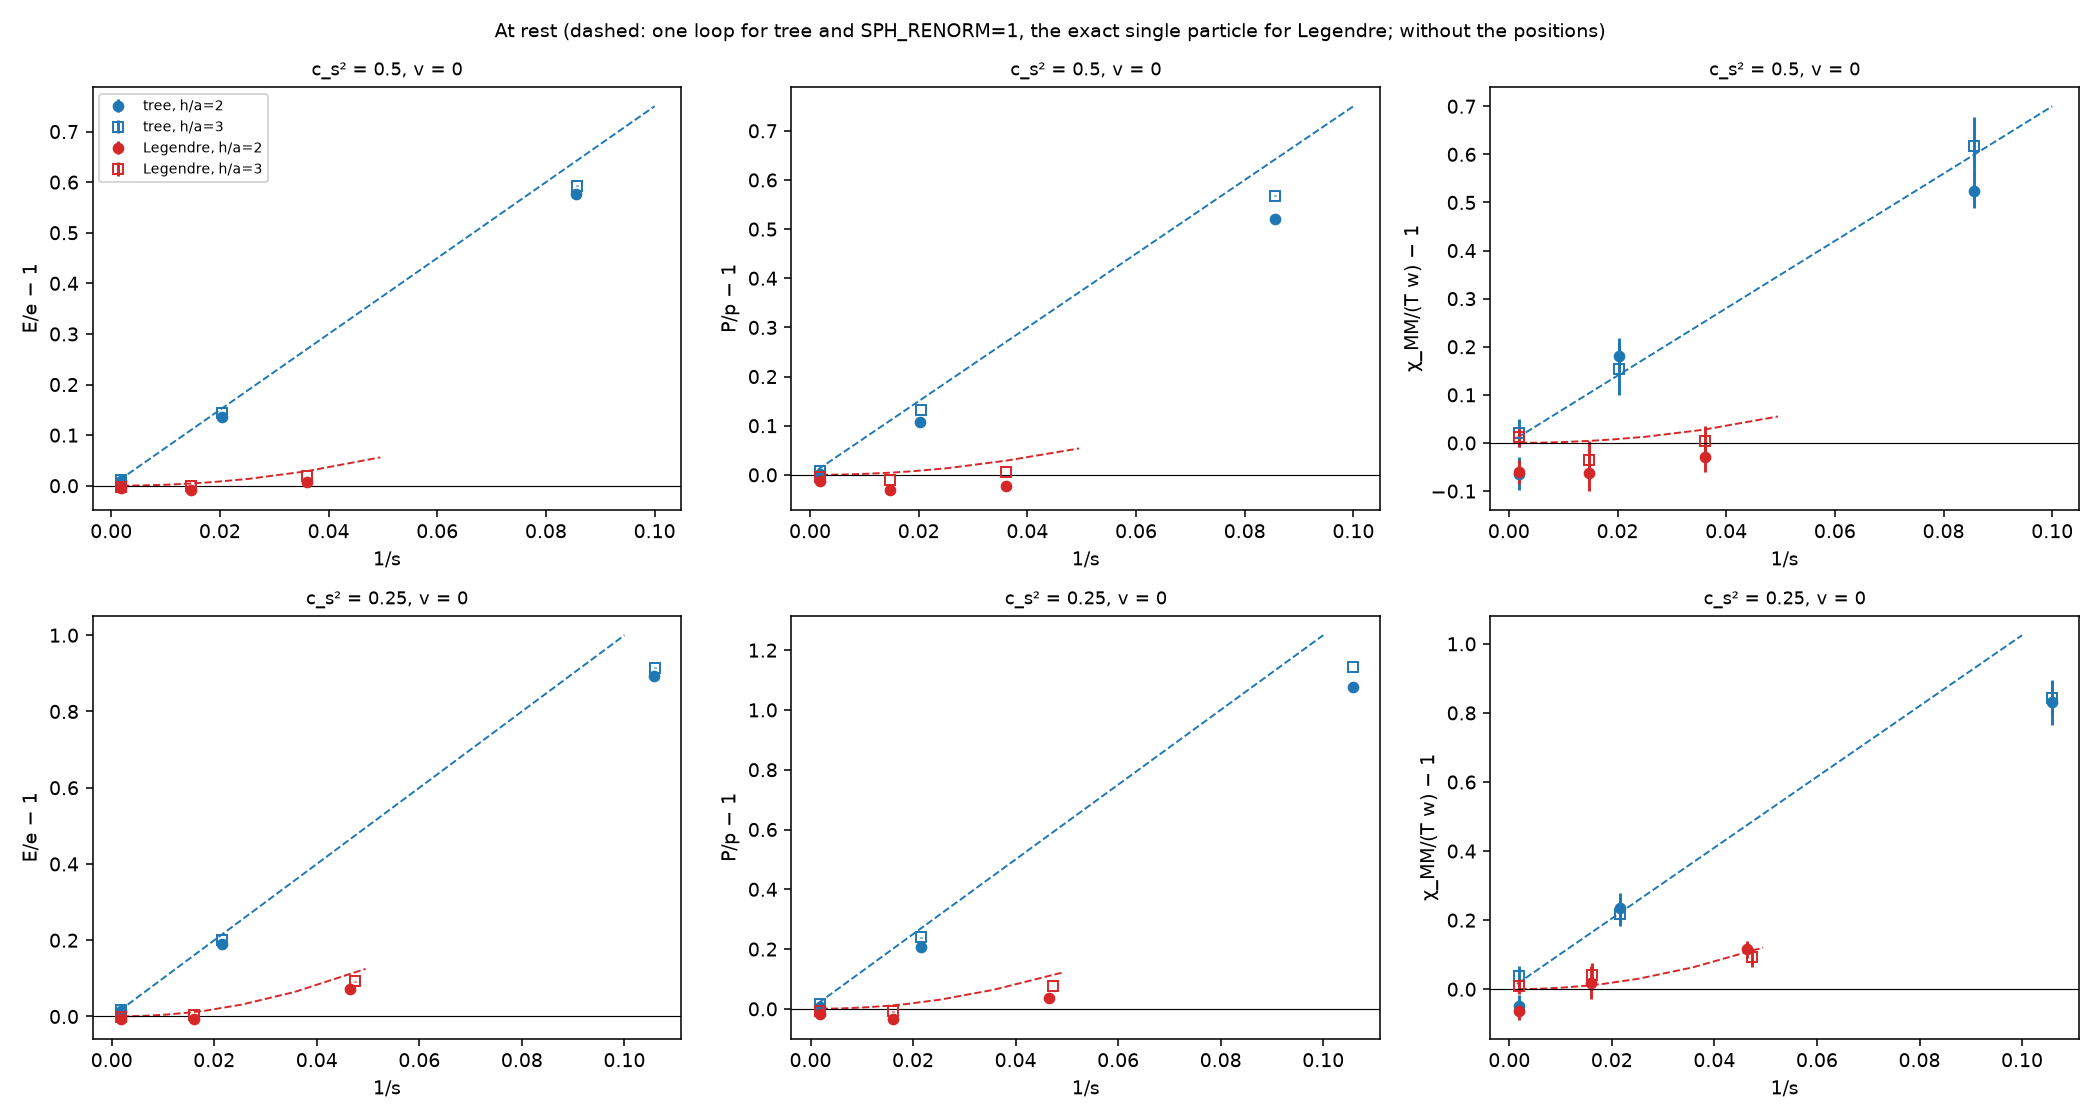
\includegraphics[width=\textwidth]{figs/legendre_EP.png}
\caption{At rest: $E/e-1$, $P/p-1$ and $\chi_{MM}/(Tw)-1$ against $1/s$, where $s$ is the measured entropy per particle, for
$c_s^2=1/2$ (top) and $1/4$ (bottom), $h/a=2$ (filled) and $3$ (open).  Blue: tree level; red: the Legendre Hamiltonian.
Dashed: the one-loop expectation for the tree level, and the exact single-particle quadrature for the Legendre Hamiltonian
(the correction of the positions is not included in either).}
\label{fig:legendre_EP}
\end{figure}

\begin{figure}[h]
\centering
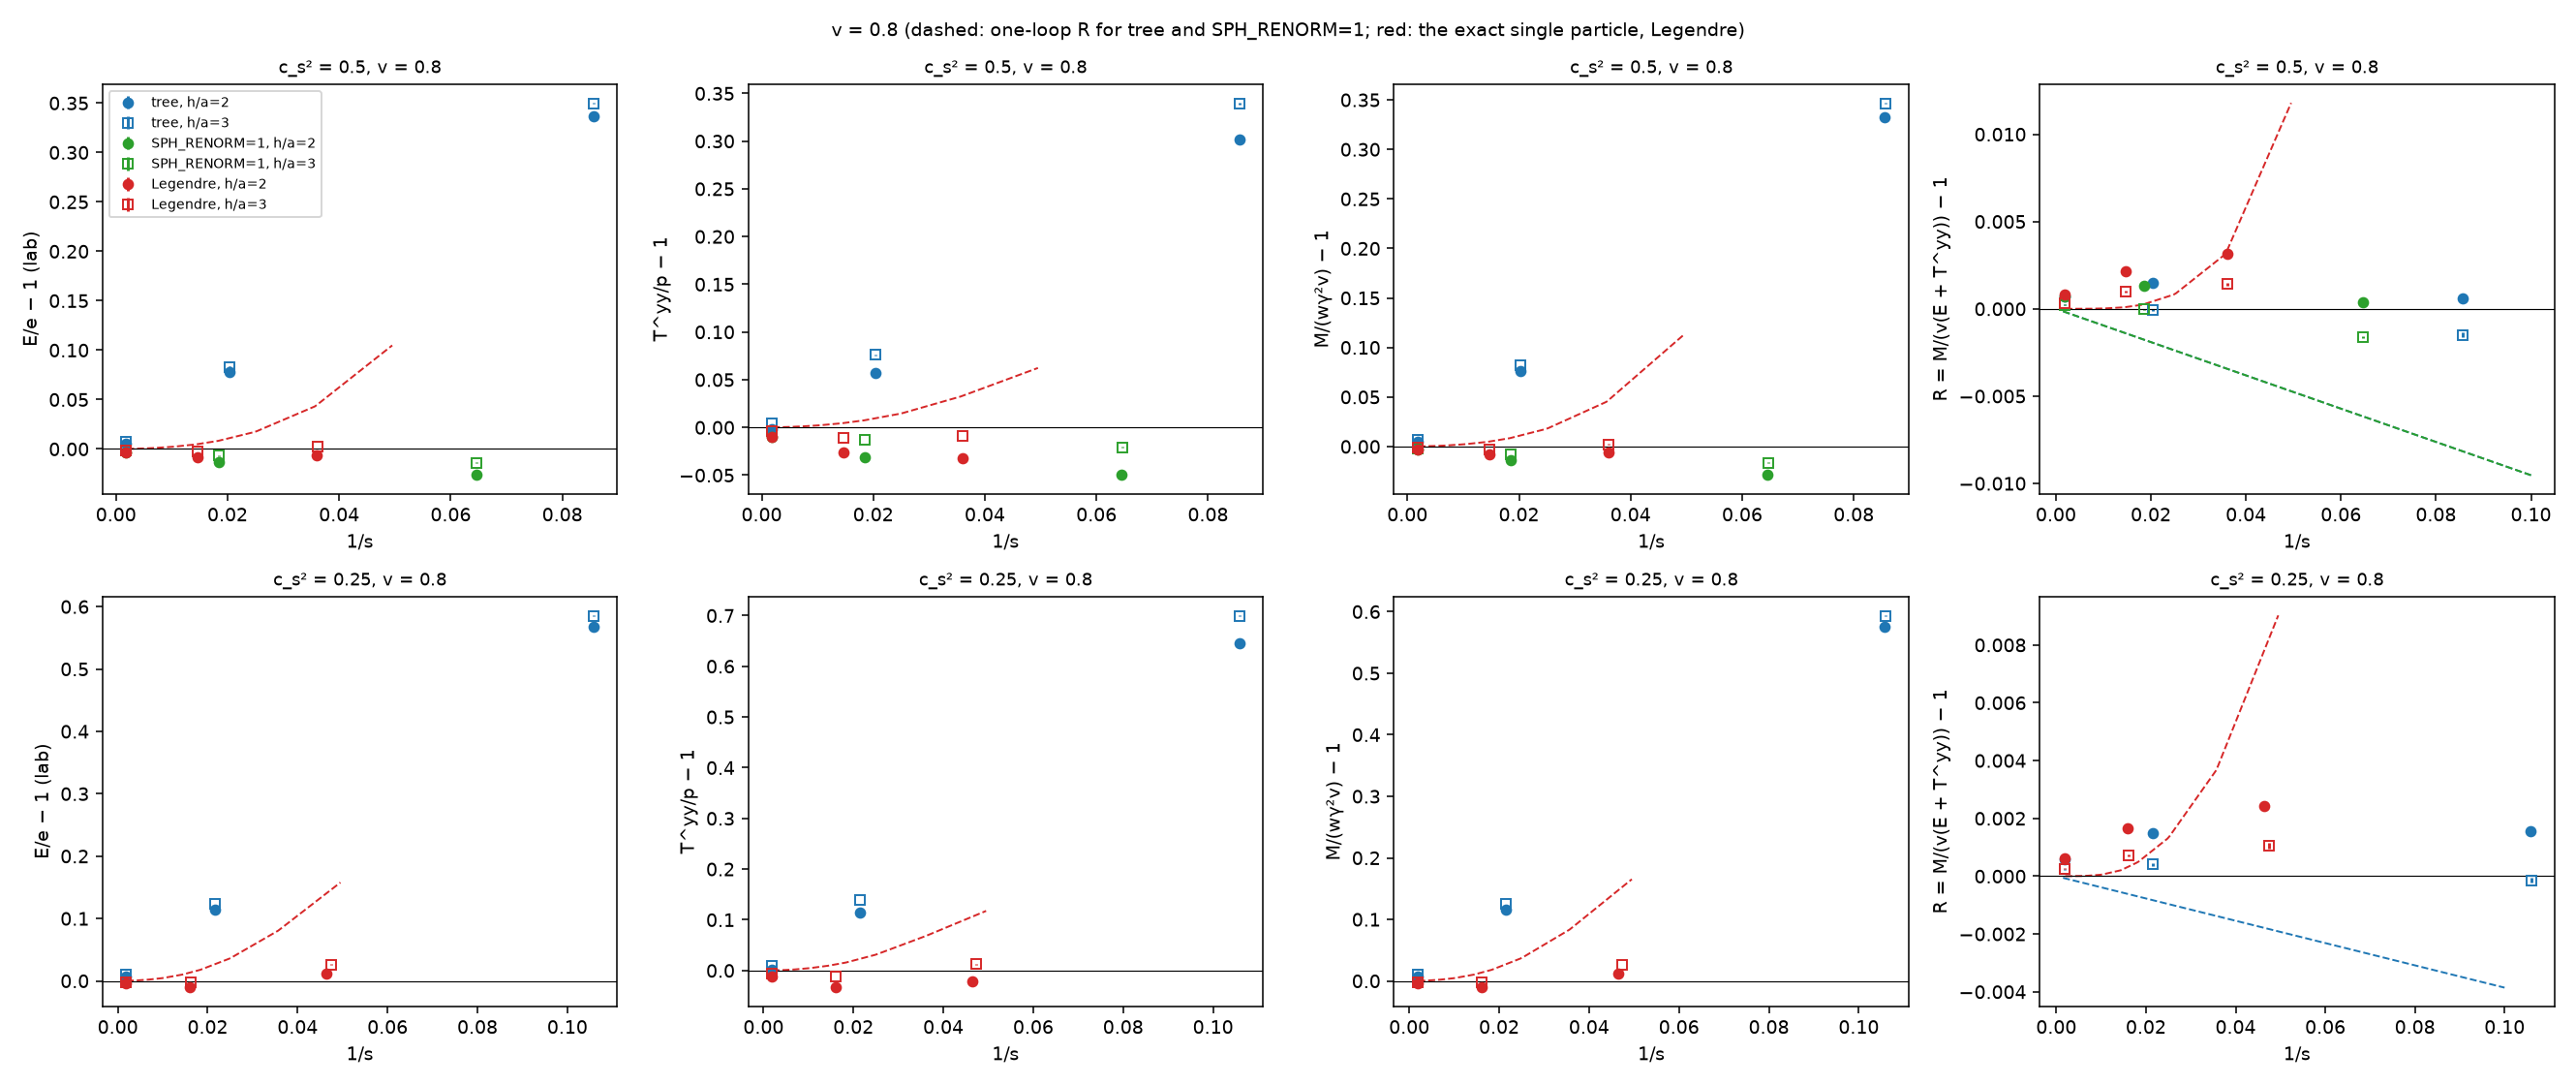
\includegraphics[width=\textwidth]{figs/legendre_moving.png}
\caption{At $v=0.8$: the lab-frame $E/e-1$, $T^{yy}/p-1$, $M/(w\gamma^2v)-1$, and $R=M/(v(E+T^{yy}))-1$ against $1/s$.  Blue: tree
level; green: \texttt{SPH\_RENORM=1}; red: the Legendre Hamiltonian.  Dashed in the last column: the one-loop
$R=-c_s^2(1-v^2)^2/((1-c_s^2v^2)s)$ for the tree level and \texttt{SPH\_RENORM=1}; red: the exact Legendre single particle.}
\label{fig:legendre_moving}
\end{figure}

\begin{figure}[h]
\centering
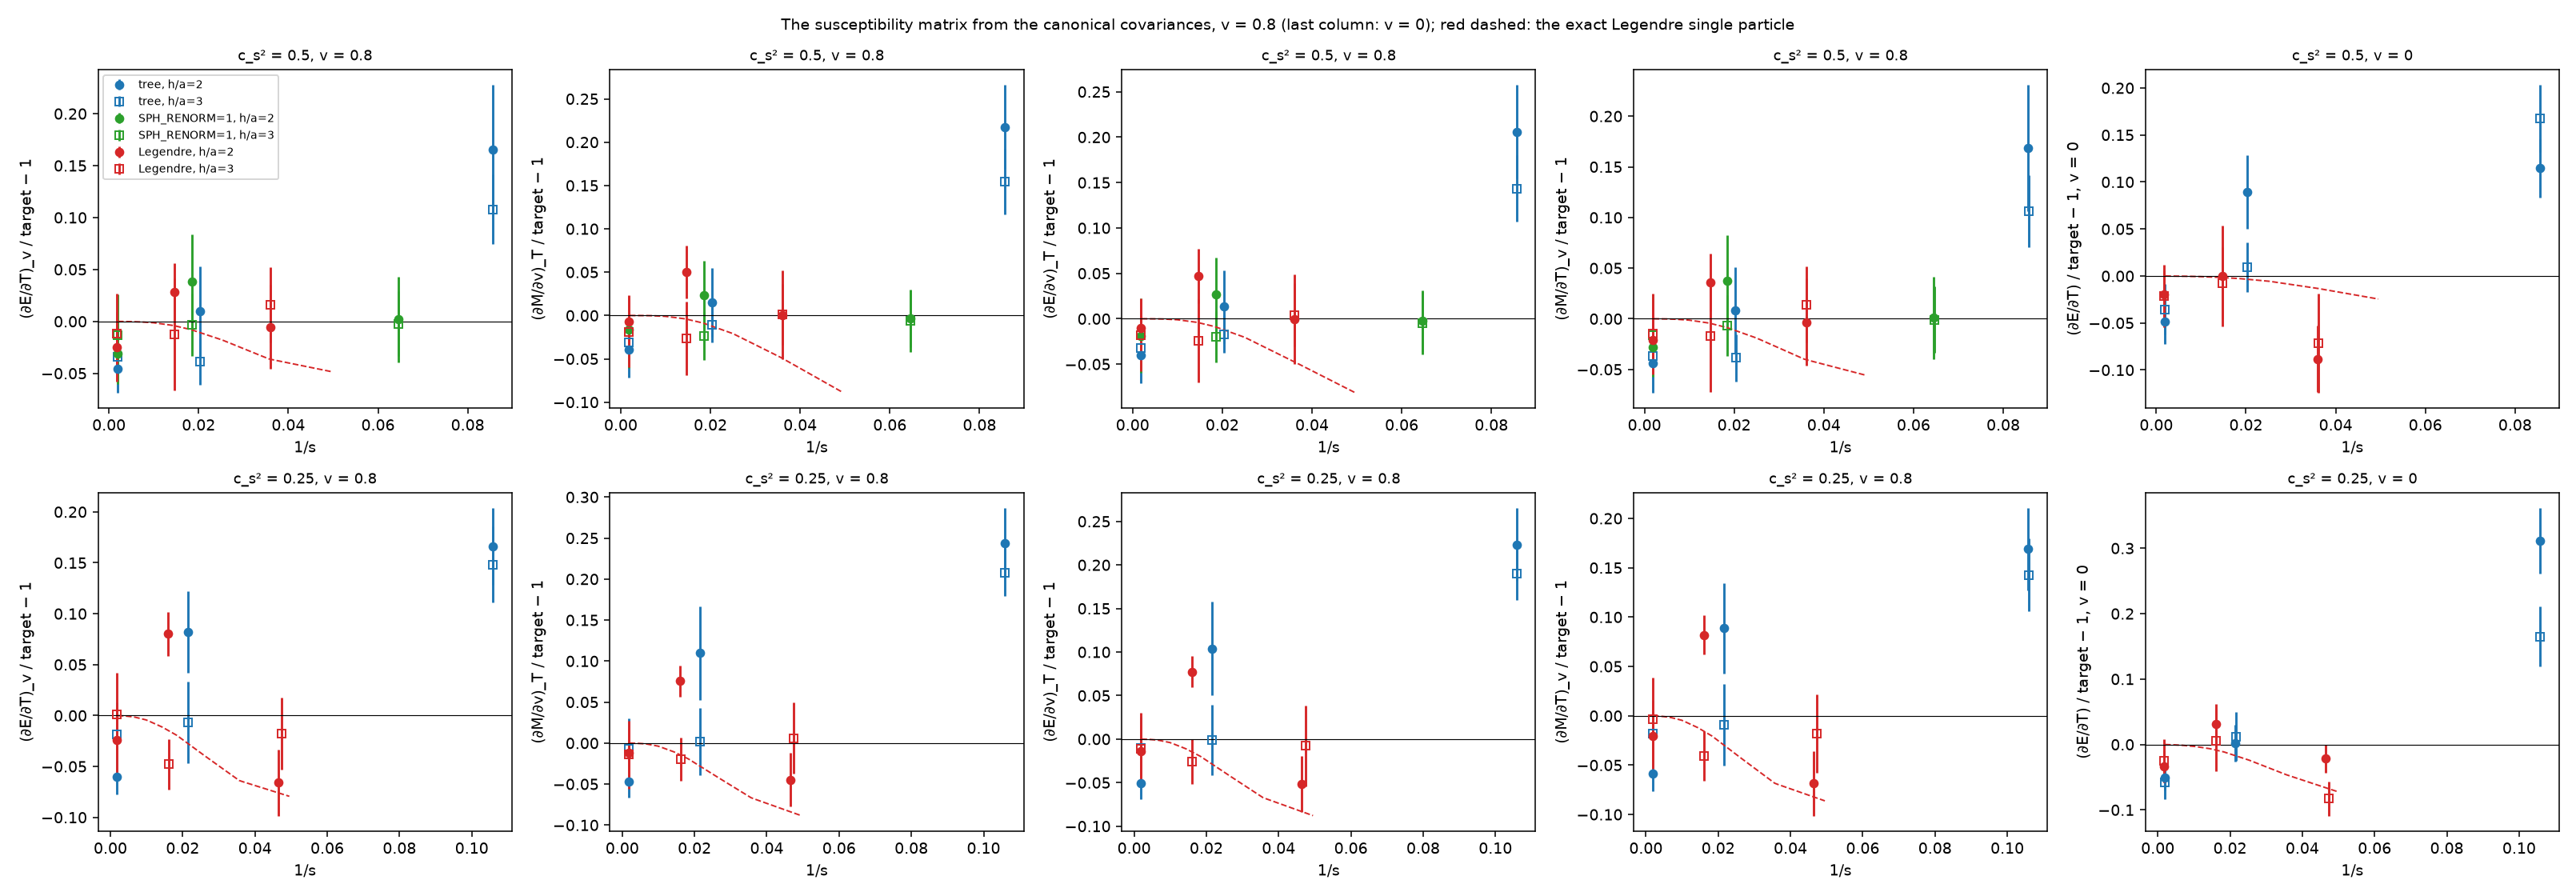
\includegraphics[width=\textwidth]{figs/legendre_chi.png}
\caption{The susceptibility matrix from the canonical covariances, relative to the target: $(\partial E/\partial T)_v$,
$(\partial M/\partial v)_T$, $(\partial E/\partial v)_T$, $(\partial M/\partial T)_v$ at $v=0.8$, and $(\partial E/\partial T)$ at
$v=0$ (last column), with jackknife errors.  Colours as in \Fig{fig:legendre_moving}; red dashed: the exact Legendre single particle.}
\label{fig:legendre_chi}
\end{figure}

\end{document}
